
\subsection{Case II : Solubility Coefficients}

The dissolution behavior of a solute in an aqueous solution is called its 
solubility. This behavior is limited by the solute's solubility limit, described  
by an equilibrium constant that depends upon temperature, water chemistry, and 
the properties of the element. 

By varying the multiplication factor applied to the expected solubility limit, 
$\langle S_i\rangle$, this analysis varied elemental solubility limits, $S_i$, 
for each isotope $i$, as detailed in Table \ref{tab:Cases}.
This method preserves, in some sense, the relative solubility 
limits between isotopes, which vary over many magnitudes.

For solubility limits below a threshold, approximately 
$1\times10^{-10}[mol\cdot m^{-3}]$, dose releases were directly 
and strongly proportional to the solubility limit. This indicated that the radionuclide 
concentration saturated the groundwater up to the solubility limit near the 
waste form.  For solubility limits above the threshold, however, further 
increase to the limit had no effect on the peak dose. This demonstrated the 
situation in which the solubility limit was so high that even complete 
dissolution of the waste inventory into the pore water was insufficient to reach 
the solubility limit.

\begin{figure}[ht]
  \centering
  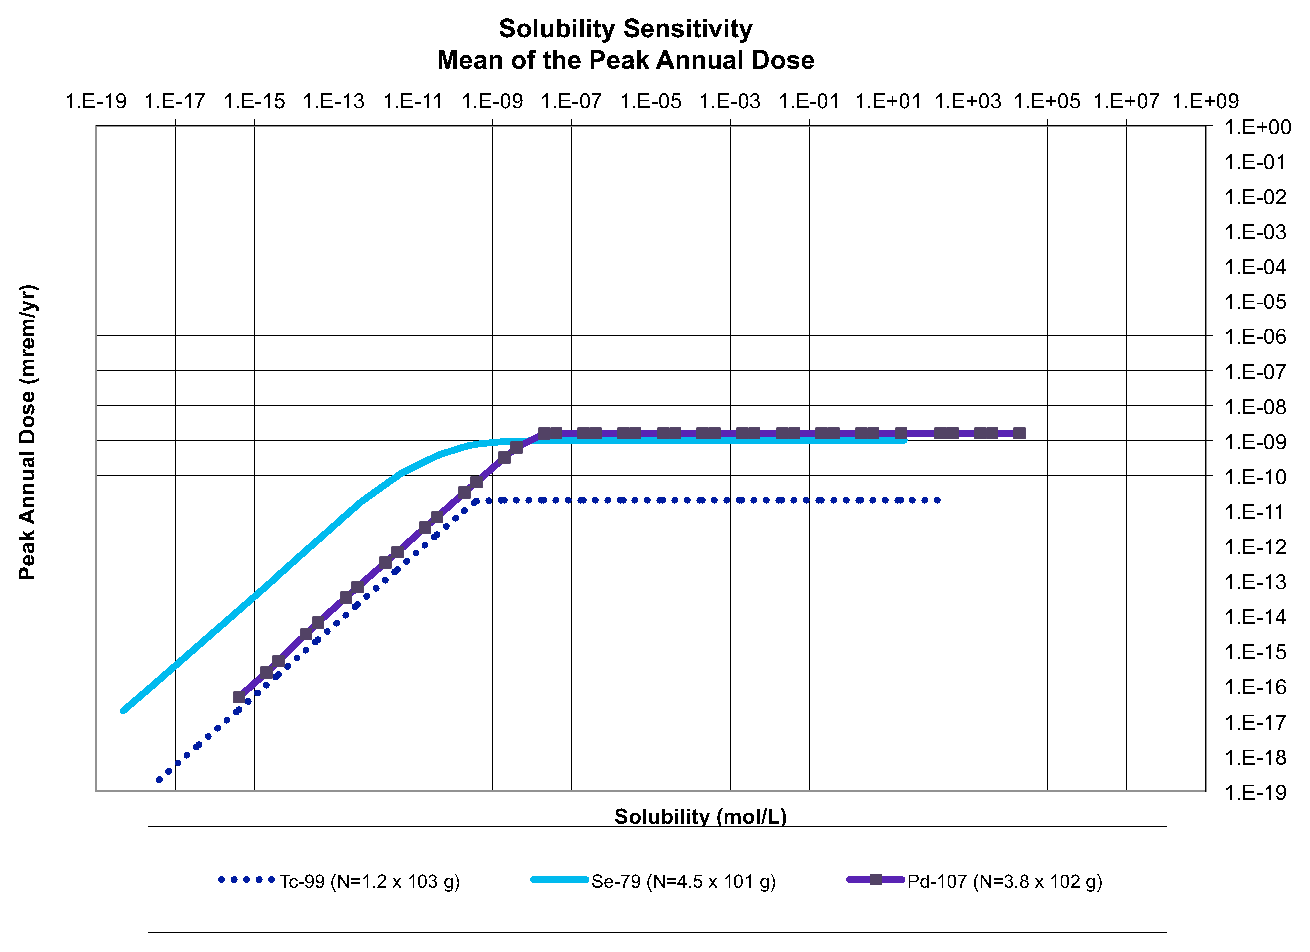
\includegraphics[width=\linewidth]{Solubility_Summary.eps}
  \caption{Solubility limit sensitivity. The peak annual dose due to an 
  inventory, 
  $N$, of each isotope.}
  \label{fig:SolSum}
\end{figure}
